\chapter{Instructions and Operands}
\label{ch:instructions-operands}

The word \code{add} does not say enough. It does not name the width, the
inputs, the destination, the condition bits, the next program counter, or the
cases in which execution cannot continue. It is a useful name for a family of
actions, not a complete account of any one action.

To move from one machine state to the next, we need an operation, an operand
form, concrete operands, and a rule that exposes every architectural effect.
The printed instruction is short. Its meaning cannot be.

\begin{keyidea}[title={An instruction meaning is a complete transition}]
An instruction does not merely calculate a value. It transforms one declared
machine state into another, or produces a declared failure. Every component
that can affect later execution belongs in that account.
\end{keyidea}

This view separates three questions that assembly listings often place on one
line. Which bytes were fetched? Which instruction instance did the decoder
produce? What does that instance do to state? A correct answer to one does not
repair an error in another.

\subsection*{From operation tables to transition rules}

An instruction table is one of computing's durable forms. It gives a short
name or bit pattern to an operation and tells a programmer which operands may
accompany it. Early manuals needed such tables because a machine could perform
only the actions supplied by its hardware. Modern architecture manuals still
use them because compatibility requires precise answers about decades of
accumulated forms.

The purpose has widened. Compilers use instruction descriptions to select and
schedule code. Assemblers turn accepted forms into bytes. Disassemblers try to
recover forms from bytes. Emulators perform the effects. Hardware verification
compares an implementation with an architectural account. Binary translators
relate one machine's transition to another's. Each consumer needs more than a
mnemonic, though not always the same more.

For this book, the central object is the architectural transition. It lies
between notation and hardware. It says what state change software is entitled
to observe while leaving circuit organization and timing to a later model.
That position gives the instruction an unusual reach: a finite rule describes
its action on every admitted state.

\begin{archive}[title={A short operation name can denote a vast table}]
At width sixty-four, one register addition rule covers more input pairs than
could be listed. The rule earns that compression by stating the arithmetic,
conditions, failures, and preserved state exactly. A short name without those
clauses compresses nothing; it merely postpones the definition.
\end{archive}

\section{From a spelling to an action}

\begin{definition}[title={Instruction instance}]
An \keyterm{instruction instance} is an operation together with one allowed
operand form and concrete operands. Its semantics gives the complete state
change for a running input state, including the next program counter and any
trapped outcome.
\end{definition}

Object \obj{A0.def.instruction} records this state-transformer view. A decoded
instruction is not the same object as its printed assembly or its instruction
bytes. Assembly is a human-readable notation. Decoding turns bytes into an
instruction instance. Semantics says what that instance does. Chapter 6 will
study the boundary between the last two.

\begin{figure}[htbp]
\centering
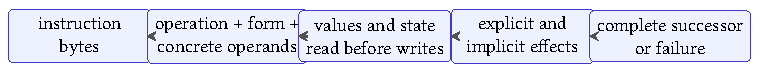
\includegraphics[width=0.94\textwidth]{figures/instruction-instance-layers}
\caption{One printed instruction conceals several contracts. Bytes select an
instance; the instance determines reads and effects; the semantics returns a
complete successor or a declared failure.}
\figalt{Instruction bytes pass through an instruction instance, old-state reads, effects, and finally a complete successor or failure.}
\label{fig:instruction-instance-layers}
\end{figure}

For deterministic A0, a fixed instruction instance and running input state
select at most one successor. We may therefore present its meaning as a
function whose result includes either an ordinary state or a trapped state.
Other machine models may use a relation and admit several successors: an
underspecified value, an external event, or a concurrent action can make more
than one next state possible. Calling both accounts semantics does not make
their proof obligations identical.

\begin{definition}[title={Deterministic instruction semantics}]
An instruction semantics is deterministic when one instruction instance and
one admitted input state never relate to two different successor states.
Existence is separate: a halted state may have no instruction successor, and
a partial model may leave some forms outside its domain.
\end{definition}

Determinism is useful because a witness state can be replayed without making
another choice. It does not imply termination of a program, successful
execution, or simplicity of an instruction. A deterministic load may trap on
one state and succeed on another. A deterministic variable-length decoder may
need several bytes before it selects its one answer.

The separation matters even when the printed text looks familiar. Two
assemblers may accept different spellings for the same decoded form. One
sequence of bytes may be illegal even though a nearby legal sequence prints a
recognizable mnemonic. A decoder can correctly identify an instruction whose
transition function is wrong. The book will test each boundary with a
different kind of control.

Consider the A0 instance \code{add r0, r1, r2}. It reads \(R[r_1]\) and
\(R[r_2]\). It adds them modulo \(2^w\), writes the result to \(R[r_0]\), sets
\(Z,N,C,V\) by the A0 addition rules, and advances \(pc\) by four modulo
\(2^w\). Other registers and data memory remain unchanged. Because the
instruction has already been decoded, no data-range trap belongs to this
particular operation.

Take width eight, \(R[r_1]=255\), and \(R[r_2]=1\). The result in \(r_0\) is
0. The zero bit \(Z\) is one, the negative bit \(N\) is zero, and the carry
bit \(C\) is one because the mathematical sum reached 256. Signed overflow
\(V\) is zero: the signed inputs are -1 and 1, whose mathematical sum is
representable. If \(pc=12\), the next sequential value is 16.

\begin{example}[title={One complete A0 addition}]
The input facts are width eight, \(R[r_1]=255\), \(R[r_2]=1\), \(pc=12\), and
a running outcome. The instruction reads \(r_1\) and \(r_2\). It writes 0 to
\(r_0\), writes \((Z,N,C,V)=(1,0,1,0)\), advances \(pc\) to 16, preserves all
other registers and data memory, and leaves the outcome running. Removing any
one of those clauses produces an incomplete transition.
\end{example}

Preservation clauses deserve to be explicit. If a rule lists only the fields
that change, a reader may infer that every unlisted field stays fixed. An
executable semantics must enforce that inference. Otherwise an implementation
could change \(r_7\) while still satisfying a postcondition that mentions only
\(r_0\) and the flags.

This worked step shows why a destination value is not the whole result. A rule
that writes 0 to \(r_0\) but leaves \(C=0\) has performed a different A0
transition. So has a rule that leaves \(pc=12\).

\section{What an operand does}

An operand is often introduced as a place where an instruction gets a value.
That account is too narrow. A destination operand names where a value goes. A
memory operand also triggers address formation and can trap. A relative target
contributes to the next program counter rather than to arithmetic data.

\begin{definition}[title={Operand form}]
An A0 \keyterm{operand form} states how an operand is obtained, whether the
instruction reads or writes it, its width, and any state effect required to
use it. A0 has register operands, signed immediate values, base-plus-offset
memory locations, and relative branch targets.
\end{definition}

Object \obj{A0.def.operand} records these four forms. An A0 immediate comes
from the signed eight-bit immediate field and is sign-extended to \(w\) bits.
A memory address adds that same signed offset to a base register. A relative
target adds four times the signed offset to the sequential address \(pc+4\).
The multiplication keeps branch targets on four-byte instruction boundaries.

The written operands need not list every state component the operation uses.
The A0 \code{add} instance prints three registers yet also writes four
condition bits and the program counter. These are \keyterm{implicit effects}:
architectural reads or writes fixed by the operation even though they are not
printed as operands.

The distinction between a printed operand and a value role prevents another
shortcut. A destination may also be a source. An address operand may read a
base register, read an offset from the instruction, access memory, and expose
a trap. A branch target may consume the current program counter even when the
assembly does not print it. Counting commas does not count semantic inputs.

\begin{table}
\centering
\caption{The four A0 operand forms and the work each form contributes.}
\begin{tabular}{p{0.15\textwidth}p{0.20\textwidth}p{0.20\textwidth}p{0.25\textwidth}}
\toprule
Form & Value source & State access & Extra rule \\
\midrule
register & named register & read or write & width \(w\) \\
immediate & instruction byte & no register read & sign extension \\
memory & base plus offset & register and bytes & range check \\
relative target & sequential \(pc\) plus offset & program counter & alignment and code range \\
\bottomrule
\end{tabular}
\end{table}

\begin{keyidea}[title={Explicit effects}]
A semantic rule must expose every architectural read, write, program-counter
change, and exceptional outcome used by its instruction form.
\end{keyidea}

Object \obj{A0.prin.explicit-effects} records this rule. It is a discipline
for the semantics, not a requirement that assembly syntax spell out every
effect.

\subsection{Well-formed operands are checked before arithmetic}

An operation name does not accept every operand tuple. A register field must
name an available register. A form may require distinct roles, a particular
width, or an immediate that fits its encoded field. A memory form may permit
only certain base and offset combinations. These restrictions define the
set of legal instruction instances.

Keeping that check separate from execution gives illegal forms an honest
home. If reserved bytes decode to no instruction, the failure belongs to
decoding. If an external API tries to construct an operand tuple that no A0
encoding can denote, the typed constructor should reject it before the step
function runs. The execution semantics need not invent behavior for an object
the instruction set excludes.

\begin{keyidea}[title={Legality precedes effect}]
First establish that the bytes select one admitted instruction instance. Then
apply the transition for that instance to state. A semantic equation for a
legal addition says nothing about a reserved encoding that resembles it.
\end{keyidea}

This distinction matters in testing. Random instruction bytes exercise the
decoder's acceptance partition. Random legal instruction instances exercise
the transition rules. Generating the second set by decoding the first is
useful, but it can miss a legal form that the decoder never emits. A complete
test plan checks the two domains and their connection.
Neither collection can establish coverage of the other merely by producing
many successful examples.

\subsection{Read old values before committing new ones}

An instruction may name the same location in more than one role. In
\code{add r0,r0,r1}, the old value of \(r_0\) is a source and \(r_0\) is also
the destination. The semantics must read the source before replacing the
destination. Otherwise the result would depend on the order in which a prose
description happened to mention its effects.

A clean rule takes a logical snapshot of every required input from the old
state. It evaluates register sources, immediate values, addresses, and any
required memory bytes against that state. Only after those operations succeed
does it commit the destination, implicit state, next program counter, and
outcome together.

\begin{figure}[htbp]
\centering
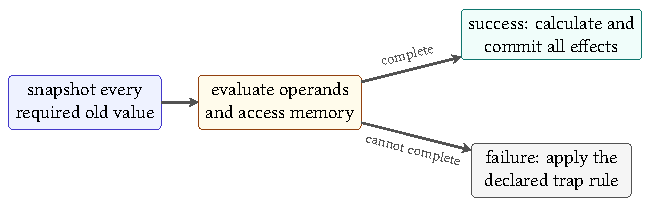
\includegraphics[width=0.88\textwidth]{figures/operand-effect-order}
\caption{Operand evaluation uses the old state. The instruction commits its
ordinary effects only after every required operand operation succeeds.}
\figalt{Old values are captured, operands and memory are evaluated, and the path then selects either all successful effects or a declared trap rule.}
\label{fig:operand-effect-order}
\end{figure}

This snapshot is semantic, not a demand that hardware copy the full state.
An implementation may forward a result, rename a register, or calculate
several pieces in parallel. It implements the rule when its architectural
successor is the same as if the inputs came from the old state and the effects
were committed according to the declared outcome.

Memory makes failure ordering visible. Suppose an instruction reads a memory
source and writes a register destination. If the address or range check fails,
the destination write does not occur under the A0 rule. A faulty
implementation that clears the destination first and discovers the bad
address second has created a successor the semantics excludes.

\begin{warning}[title={Prose order is not effect order}]
The sentence ``write the destination and advance the program counter'' does
not license an implementation to expose the first write when a later required
operation fails. A semantic rule must state which effects commit together and
which state accompanies each failure.
\end{warning}

For instructions with two memory operands or implicit stack effects, the
same issue becomes more demanding. The rule must identify every access,
their ordering, and the state retained on failure. A0 avoids those forms in
its first instruction set, but the method is already in place for the selected
x86-64 cases that combine more work in one instruction.

\section{One step}

A running machine does not execute a mnemonic in isolation. It uses the
program counter to fetch instruction bytes, decodes those bytes, and applies
the decoded instruction's transition.

\begin{figure}[htbp]
\centering
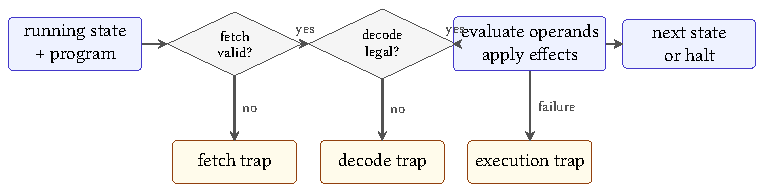
\includegraphics[width=0.98\textwidth]{figures/a0-single-step}
\caption{One A0 step keeps fetch failure, decode failure, and execution failure
distinct. Only the successful path reaches the ordinary next state.}
\figalt{A running state passes through fetch, decode, and effects, with separate trap exits at all three stages.}
\label{fig:a0-single-step}
\end{figure}

\begin{definition}[title={A0 single step}]
An A0 \keyterm{single step} takes a running state and a program. It checks the
program counter and fetch range, decodes one four-byte instruction, and
applies that instruction's complete transition. A fetch or decoding failure
produces a trapped state. A halted or trapped state has no successor.
\end{definition}

Figure~\ref{fig:a0-single-step} is ordered. The machine cannot evaluate an
operand from an instruction that did not decode. It cannot decode bytes that
were not fetched from a valid code range. If operand evaluation traps, later
writes in the instruction do not occur unless the instruction rule explicitly
says otherwise. This order is part of the semantics, not an implementation
optimization.

\begin{warning}[title={Three failures, three debugging questions}]
A fetch trap asks whether the program counter names available instruction
bytes. A decode trap asks whether those bytes form one legal A0 encoding. An
execution trap asks whether a legal decoded instruction can complete on this
state. Collapsing all three into ``bad instruction'' hides which rule failed.
\end{warning}

Object \obj{A0.def.step} records this relation. The definition names decoding
before Chapter 6 teaches the encoding because execution needs the boundary to
exist. For hand traces in Part I, we will print both the four bytes and their
decoded form so the decoding step is visible without becoming the lesson.

The ordinary next address is \(pc+4\) modulo \(2^w\). A branch or jump may
replace it with a relative target. A trap records its reason and prevents a
later instruction from running. These three cases are part of the transition,
not annotations added after the register calculation.

Two simple attacks test whether a proposed step rule has hidden omissions.
First, change the expected carry bit while leaving the destination correct.
A complete-state check must reject the step. Second, leave the program counter
unchanged after a normal \code{add}. A checker that looks only at \(r_0\) will
miss the error; a checker for the whole A0 transition must not.

\subsection{Read and write footprints summarize dependence}

The \keyterm{read footprint} of an instruction on a state is the architectural
information needed to determine its successor. The \keyterm{write footprint}
is the set of components that may differ in that successor. For
\code{add r0,r1,r2}, the read footprint contains the two source registers,
the program counter, and enough outcome state to require a running input. Its
write footprint contains \(r_0\), the four condition bits, and the program
counter.

Footprints are more exact than lists of printed operands and less cumbersome
than repeating the complete transition. They expose data dependence: a later
instruction depends on an earlier one when it reads a component the earlier
one may write. They also support frame reasoning: everything outside the
write footprint must retain its old value unless the failure rule says
otherwise.

The footprint can depend on the state. A memory operand's byte addresses come
from register values. A conditional branch reads the predicate needed to
choose one path, while the successor address depends on that choice. For a
conservative static analysis, one may use a larger footprint that contains
every possible address or component. That is safe for detecting possible
dependence, but it may report interactions that no admitted state can realize.

\begin{proofkit}[title={Equal reads give equal deterministic effects}]
Fix one deterministic instruction instance. If two admitted input states
agree on its complete read footprint, operand evaluation receives the same
values and makes the same success or failure decisions. The instruction then
calculates equal values for its write footprint. Components outside that
footprint retain their respective old values. The full successors are equal
only if the old states also agree on those preserved components.
\end{proofkit}

The last sentence matters. Agreement on what an instruction reads is enough
to make its newly calculated effects agree. It is not enough to make complete
successor states equal when unrelated old state already differed. Chapter 11
will turn that distinction into observations and state relations.

\section{Three value roles, two printed operands}

The two companion architectures make operand roles visible in different ways.
A later RV64 integer addition will use a form such as
\code{add rd, rs1, rs2}. The destination name is separate from the two source
names. The selected base form does not write an x86-style condition-code
register.

A later x86-64 register addition will use a two-operand form such as
\code{add rax, rbx}. The destination \code{rax} is also the first source. The
instruction reads the old values of \code{rax} and \code{rbx}, writes the sum
to \code{rax}, and changes selected status flags.

One spelling therefore names three register roles with three operands. The
other names three value roles with two operands and adds implicit condition
writes. This is a concrete comparison of operand and state design. Calling
one RISC and the other CISC may place the examples in historical families; it
does not supply either transition rule.

Here is the reader argument that keeps the extra state honest. Suppose two
instructions start from the same state and both leave 2 in their destination.
One leaves \(Z=0\), while the other leaves \(Z=1\). Their output states differ
in the \(Z\) component. They may agree under an observation of the destination
alone, but they are not equal state transformers. A following branch that
reads \(Z\) can expose the difference.

The comparison also warns against translating syntax directly. To relate the
two additions, we must first decide where the three input and output values
live, then account for every extra state component. A destination-only
observation may permit a relation that a flag-sensitive context would reject.
The choice belongs in the claim, not in an informal declaration that both
lines are additions.

Instruction forms also differ in where they place constants and addresses.
An RV64 immediate form may carry a constant in fixed instruction fields and
write a destination distinct from its source. An x86-64 form may allow an
immediate or memory operand in a position whose other role can be a register.
These are encoding and operand choices. The arithmetic relation can still be
the same after widths, source values, destinations, and extra effects are
aligned.

Implicit operands deserve the same treatment as implicit conditions. A stack
operation may read and write a stack pointer that the assembly does not print.
A procedure-return instruction may obtain its target from a fixed register or
memory location. Some multiply and divide forms use architecturally selected
register pairs. These choices can make a short line depend on substantial
state.

\begin{sidebar}[title={Fewer printed operands do not mean fewer inputs}]
Assembly syntax is a notation optimized for programmers who know the
architecture's conventions. It may omit a fixed register, a condition-code
write, a stack update, or the ordinary next address. Semantic comparison must
restore those facts before counting sources, destinations, or effects.
\end{sidebar}

\begin{tryit}[title={Read sets before arithmetic}]
For each of these A0 forms—\code{add r0,r1,r2}, \code{movi r0,-1},
\code{load r0,[r1+4]}, and \code{branch.eq +2}—list the complete read set and
write set before calculating any values. Include implicit state and possible
outcomes. Which two forms can trap after successful decoding?
\end{tryit}

\section{Instructions in sequence}

If instruction \(i\) takes \(S_0\) to a running state \(S_1\), and instruction
\(j\) takes \(S_1\) to \(S_2\), then the sequence \(i;j\) has taken \(S_0\) to
\(S_2\). This is ordinary function composition with an outcome check between
the functions.

If \(i\) halts or traps, there is no \(S_1\) on which \(j\) may run. A model
that applies \(j\) anyway has not found an unusual execution of A0. It has
defined another machine. This small point will become important when bounded
execution distinguishes a stopped trace from one that merely reached its
step limit.

Memory operands add a second source of interruption. Before an arithmetic
operation can use a memory value, the machine must form the address and
complete the load. If that access traps, the main arithmetic write does not
occur. The order of these effects belongs in the instruction rule.

\begin{proofkit}[title={\iconProofKit\ Composition needs a running middle state}]
Assume instruction \(i\) takes \(S_0\) to a running state \(S_1\), and
instruction \(j\) takes \(S_1\) to \(S_2\). Then the two-instruction sequence
is defined by applying \(j\) to the output of \(i\). If \(i\) instead returns
a halted or trapped state, the premise needed to apply \(j\) is false. The
sequence stops with the first outcome; it does not possess a hidden second
transition.
\end{proofkit}

The result is a partial form of composition. Each decoded instruction has a total
rule over the running states admitted by its operands: it returns a next state
or a trapped state. Program sequencing adds an outcome guard. Later trace
definitions will make that guard visible at every adjacent pair.

When all required middle states are running, deterministic composition is
associative. Grouping \((i;j);k\) or \(i;(j;k)\) produces the same successive
states because both groupings apply \(i\), then \(j\), then \(k\). Parentheses
organize the argument; they do not change the instruction order. The outcome
guard must still be checked after each step.

Footprints explain when order can change. Two instructions with disjoint
write footprints are not automatically interchangeable: one may write a
component the other reads, both may trap under different premises, or their
program-counter effects may select different code. For straight-line local
reasoning, a sufficient commutation argument must show that neither write
meets the other's reads or writes and that both outcome conditions remain the
same in either order.

These footprint intersections are the semantic root of familiar instruction
hazards. A read-after-write
dependence carries a value forward. A write-after-read dependence can make
reordering destroy an old value before it is consumed. A write-after-write
dependence makes final state depend on which write comes last. Hardware may
execute internally in another schedule, but retirement must preserve the
architectural result required by the machine model.

The statement is deliberately broader than registers. Condition bits,
memory bytes, program counters, and outcomes can create the same dependencies.
An optimizer that sees only named registers may move an addition across a
flag-reading branch or move a load across an overlapping store. The assembly
still looks plausible. The state transition has changed.

\section{The implementation boundary}

An Axeyum implementation must join the state, decoder, operand rules, and
instruction transitions into one reusable A0 step. Object
\obj{OP.a0.step} records that obligation. Its controls must include the wrong
destination, a missing condition write, a wrong sequential program counter, a
wrong branch target, reserved encoding fields, and attempted execution after
halt or trap.

The corresponding introductory Axeyum route should begin with execution, not
with a solver. A reader should construct one width-eight state and one decoded
\code{add}, run the public step function, and inspect the complete output.
Only then should a relation ask whether a proposed shortcut agrees for every
allowed input. A returned counterexample must replay through that same step
function. A no-counterexample result must name the formula and checking route
before it can support a machine-proof claim.

The public data model should keep the layers in
Figure~\ref{fig:instruction-instance-layers} separate. A decoded instance
contains an operation and typed operands, not a closure supplied by Python.
The Rust semantics matches that closed instruction type and returns a complete
state result. Serialization records enough information to reconstruct both
objects without accepting a printed mnemonic as authority.

One useful introductory display is a state diff paired with the full-state
record. The diff teaches which components changed. The full record lets the
checker establish preservation of everything else. If the artifact stores
only the diff, a missing illicit write is indistinguishable from a preserved
component.

Controls should attack one layer at a time. Change bytes while retaining the
printed instance. Change an operand register while retaining the operation.
Change one implicit condition while retaining the destination. Corrupt the
next program counter while retaining all arithmetic. A route that rejects
only the last mutation has not checked decoding or operand binding.

\begin{sidebar}[title={A useful first mutation}]
Change only the sequential update from \(pc+4\) to \(pc+1\). A test at
\(pc=0\) catches the immediate error. A stronger route quantifies over every
allowed running state and shows that destination arithmetic cannot conceal the
wrong next address. The mutation is useful because it preserves the tempting
part of the result.
\end{sidebar}

The implementation does not accompany this draft. The worked addition is a
reader execution of the printed A0 definition, not evidence that a general
step function has run over every state. When the package exists, its output
must agree with these rules and its controls must fail for the stated reasons.

Registers and immediates keep an instruction's values close at hand. A memory
operand does not. It turns one step into a claim about addresses, byte order,
valid ranges, overlap, and failure. We need to construct that part of the
machine before we can safely compose programs that touch it.
The next chapter therefore treats a memory access as a checked state movement,
not as a bracketed spelling around an address.

\section{Exercises}

\begin{enumerate}
\item \textbf{Execute.} At width eight, run
\code{add r0, r1, r2} from \(R[r_1]=127\), \(R[r_2]=1\), and \(pc=20\).
Compute \(r_0,Z,N,C,V,\) and the next \(pc\).
\item \textbf{Break.} Alter exactly one component of your answer to the first
exercise. State an observation that would miss the error and the smallest
observation that would catch it.
\item \textbf{Prove.} Show that if a first instruction traps, the two-step A0
sequence has no state produced by the second instruction. Identify the outcome
rule on which the argument depends.
\item \textbf{Transfer.} Write the value roles for the three-operand RV64
addition pattern and the two-operand x86-64 pattern. Do not compare their
complexity; compare what each form reads and writes.
\item For \code{movi r3,-1}, state where the immediate originates and how it
becomes a width-\(w\) word. Explain why it is part of the instruction instance
but not a register in the input state.
\item Design a negative control for a step implementation that incorrectly
advances \(pc\) by one byte instead of four. Give the starting \(pc\), expected
result, and bad result.
\item \textbf{Execute.} Give four legal instruction bytes and a matching
decoded A0 \code{add}. Walk through every box in
Figure~\ref{fig:a0-single-step}, including the checks that succeed.
\item \textbf{Break.} Keep the decoded operation and all explicit operands
correct, but omit one implicit write. Construct a following instruction that
can expose the omission.
\item \textbf{Prove.} Show that two state transformers equal on every complete
running state remain equal after composition with the same deterministic
suffix, provided both produce running middle states.
\item \textbf{Transfer.} For one paired addition form, state the weakest
observation under which it could refine A0 addition and one surrounding
context that requires a stronger observation.
\end{enumerate}
